% -- Anfang Präambel
\documentclass[german,  % Standardmäßig deutsche Eigenarten, englisch -> english
parskip=full,  % Absätze durch Leerzeile trennen
%bibliography=totoc,  % Literatur im Inhaltsverzeichnis (ist unüblich)
%draft,  % TODO: Entwurfsmodus -> entfernen für endgültige Version
]{scrartcl}
\usepackage[utf8]{inputenc}  % Kodierung der Datei
\usepackage[T1]{fontenc}  % Vollen Umfang der Schriftzeichen
\usepackage[ngerman]{babel}  % Sprache auf Deutsch (neue Rechtschreibung)

% Mathematik und Größen
\usepackage{amsmath}
\usepackage[locale=DE,  % deutsche Eigenarten, englisch -> US
separate-uncertainty,  % Unsicherheiten seperat angeben (mit ±)
]{siunitx}
\usepackage{physics}  % Erstellung von Gleichungen vereinfachen
\usepackage{yfonts}  % Frakturschrift für Real- und Imaginärteil komplexer Größen

\usepackage{graphicx}  % Bilder einbinden \includegraphics{Pfad/zur/Datei(ohne Dateiendung)}

% Gestaltung
%\usepackage{microtype}  % Mikrotypographie (kann man am Ende verwenden)
\usepackage{booktabs}  % schönere Tabellen
%\usepackage[toc]{multitoc}  % mehrspaltiges Inhaltsverzeichnis
\usepackage{csquotes}  % Anführungszeichen mit \enquote
\usepackage{caption}  % Anpassung der Bildunterschriften, Tabellenüberschriften
\usepackage{subcaption}  % Unterabbildungen, Untertabellen, …
\usepackage{enumitem}  % Listen anpassen
\setlist{itemsep=-10pt}  % Abstände zwischen Listenpunkten verringern

% Manipulation des Seitenstils
\usepackage{scrpage2}
% Kopf-/Fußzeilen setzen
\pagestyle{scrheadings}  % Stil für die Seite setzen
\clearscrheadings  % Stil zurücksetzen, um ihn neu zu definieren
\automark{section}  % Abschnittsnamen als Seitenbeschriftung verwenden
\ofoot{\pagemark}  % Seitenzahl außen in Fußzeile
\ihead{\headmark}  % Seitenbeschriftung mittig in Kopfzeile
\setheadsepline{.5pt}  % Kopzeile durch Linie abtrennen

\usepackage[hidelinks]{hyperref}  % Links und weitere PDF-Features

% TODO: Titel und Autor, … festlegen
\newcommand*{\titel}{Quantenanalogie}
\newcommand*{\autor}{Tom Drechsler, Konstantin Schmid}
\newcommand*{\abk}{QA}
\newcommand*{\betreuer}{Max Mende}
\newcommand*{\messung}{22.11.2019}
\newcommand*{\ort}{REC/D301}

\hypersetup{pdfauthor={\autor}, pdftitle={\titel}}  % PDF-Metadaten setzen
\begin{document}
% automatischen Titel konfigurieren
\titlehead{Fortgeschrittenen-Praktikum \abk \hfill TU Dresden}
\subject{Versuchsprotokoll}
\title{\titel}
\author{\autor}
\date{\begin{tabular}{ll}
Protokoll: & \today \\
Messung:  & \messung \\
Ort: & \ort \\
Betreuer:  & \betreuer
\end{tabular}}

% -- Ende Präambel


\begin{titlepage}
\maketitle  % Titel setzen
\tableofcontents  % Inhaltsverzeichnis
\end{titlepage}

% Text Anfang
\section{Versuchsziel und Überblick}
Ziel des Versuchs ist es Quantenphysik einfach zu erklären und anschaulich zu interpretieren. Grundlage dafür bietet die Überlegung, dass Elektronen Materiewellen sind und bei diesen somit auch die Phänomene Reflexion, Beugung, Brechung, Überlagerung, Interferenz und stehende Wellen auftreten. Somit sollte es auch möglich sein dies mit Wellen, deren Wellenlängen in einem vergleichsweise makroskopischen Bereich liegen (für z.B Schall einige cm), zu rekonstruieren.
\newline Mit Hilfe eines Lautsprechers sollen Schallwellen erzeugt werden, die in einen Resonator eingesperrt werden. Dieser hat je nach zu betrachtender Analogie eine andere Form, die im jeweiligen Versuchsunterpunkt diskutiert werden wird. Danach wird die Ausbildung stehender Wellen untersucht, da diese unter gleichen Randbedingungen die jeweilige quantenmechanische Lösung gut modellieren. Die gebundenen Lösungen der Schrödinger-Gleichung sind nämlich stehende Wellen.

\section{Theoretische Grundlagen}

\subsection{Quantenmechanisches Teilchen in einer Box}
In diesem Teilversuch wird ein Röhrenresonator verwendet. Dies ist ein geschlossener Hohlzylinder der Länge $L$ mit einem Lautsprecher an einem Ende. Bei einige Frequenzen $f$ stellen sich stehende Wellen ein. Dies kann durch folgende Gleichung, die sogenannte Resonanzbedingung, beschrieben werden:
\begin{align}
\label{1}2L = n \, \frac{c}{f} = n\lambda
\end{align}
Hierbei ist $c$ die Schallgeschwindigkeit, $\lambda$ die Wellenlänge und $n  \in N_{>0}$. Dies kann Analog zu den Lösungen für ein quantenmechanisches Teilchen in einem unendlich hohen Potentialtopf betrachtet werden.
\newline
\newline Nun gilt es sich die Differentialgleichungen und deren Lösungen beider Situationen anzuschauen, um diese zu vergleichen und sich so die Qualität und den Gültigkeitsbereich der Analogie klarzumachen.
\newline
\newline Die Wellengleichung für den Luftdruck resultiert aus der linearisierten Eulergleichung und der Kontinuitätsgleichung und lautet:
\begin{align}
\frac{\partial^2p}{\partial t^2}=\frac{1}{\rho \kappa} \Delta p
\end{align}
$\rho$ ist die Massendichte der Luft, $t$ die Zeit, $\kappa$ die Kompressibilität und $p$ der Luftdruck. Als Ansatz zur Lösung dieser partiellen Differentialgleichung verwendet man:
\begin{align}
p(x)=p_0 \, \cos(kx-\omega t +\alpha)
\end{align}
Es wurde dabei bereits angenommen, dass ein quasi-eindimensionales Problem betrachtet wird. $p_0$ ist dabei die Amplitude. 
Nun muss man noch berücksichtigen, dass eine Überlagerung von nach rechts und nach links laufender Welle stattfindet. Die Funktion lautet daher:
\begin{align}
p(x)=\frac{1}{2}\,p_0 \, \cos(kx-\omega t -\alpha)
\end{align}
Die Superposition von nach rechts und nach links laufender Welle lautet dann unter Ausnutzung der Rechenregeln für Sinus und Cosinus:
\begin{align}
p(x)=p_0 \, \cos(kx+\alpha)\, \cos(\omega t)
\end{align}
Durch Betrachtung der Randbedingungen $\frac{dp}{dx}\left(0\right)=0$ und $\frac{dp}{dx}\left(L\right)=0$ ergeben sich $\alpha=0$ und $k =\frac{n \pi}{L}$.
\newline
\newline In der Quantenmechanik betrachten wir die zeitunabhängige Schrödinger-Gleichung:
\begin{align}
\label{sgl}E\Psi(\vec{r}) = -\frac{\hbar^2}{2m} \Delta \Psi(\vec{r}) + V(\vec{r})\Psi(\vec{r},t)
\end{align}
Für den eindimensionalen unendlich hohen eindimensionalen Potentialtopf ist das Potential $V(x)$ definiert durch:
\begin{align}
V(x)=
  \begin{cases}
        \infty & \text{für }x\leq 0\\
	0 & \text{für } 0<x<L\\
\infty &  \text{für } x\geq L
  \end{cases}
\end{align}
Damit reduziert sich (\ref{sgl}) innerhalb des Potentialtopfes zu:
\begin{align}
E\Psi(x) = -\frac{\hbar^2}{2m} \Delta \Psi(x)
\end{align}
Die Lösungen dieser Gleichung haben aufgrund von Normierung dann die Form:
\begin{align}
\Psi(x)=\sqrt{\frac{2}{L}}\,\sin(kx+\alpha)
\end{align}
Durch Multiplikation mit einem Phasenfaktor erhält man daraus die zeitabhängige Lösung:
\begin{align}
\Psi(x,t)=\sqrt{\frac{2}{L}} \, \sin(kx+\alpha) \, e^{i \omega t}
\end{align}
%hier fehlt noch der vergleich

\subsection{Analogon zum Wasserstoffatom}
Für den zweiten Teilversuch wird ein Kugelresonator benötigt. Dieser besteht aus zwei Halbkugeln. In der oberen ist ein Mikrophon integriert und in der unteren ein Lautsprecher. Die beiden Hemisphären kann man gegeneinander verdrehen und dabei die Amplituden in Abhängigkeit vom Winkel messen.
\newline
\newline In der Quantenmechanik können wir als Ansatz für das Potential in der Schrödinger-Gleichung nun das Coulomb-Potential $-\frac{e^2}{r}$ verwenden, da es sich um ein Ein-Elektronen-System handelt. Zur Lösung muss man Kugelkoordinaten einführen und den Separationsansatz $\psi(r, \theta, \varphi) = Y^{m}_{l}(\theta, \varphi) \, R_{l}(r)$ betrachten. Daraus ergeben sich zwei Gleichungen:
\begin{align}
\label{kugelfl}-\bigg \lbrack \frac{1}{\sin(\theta)} \frac{\partial}{\partial \theta} \bigg(\sin(\theta) \frac{\partial}{\partial \theta} \bigg) + \frac{1}{\sin^2(\theta)} \frac{\partial^2}{\partial \varphi^2} \bigg \rbrack Y^{m}_{l}(\theta, \varphi) &= l(l+1) Y^{m}_{l}(\theta, \varphi) \\
-\frac{\hbar^2}{2mr} \frac{\partial^2}{\partial r^2} r R(r) - \frac{l(l+1)\hbar^2}{2mr^2} R(r)-\frac{e^2}{r} &= ER(r)
\end{align}
Die Lösungen der ersten, winkelabhängigen Gleichung sind die Kugelflächenfunktionen.
\newline
\newline Als Gleichung für den Druck  müssen wir die Helmholtz-Gleichung betrachten:
\begin{align}
-\frac{\omega^2}{c^2} \, p(\vec{r}) = \Delta p(\vec{r})
\end{align}
Dies wird nach Umformung in Kugelkoordinaten und mit dem Separationsansatz $p(r, \theta, \varphi) = Y^{m}_{l} \, f(r)$ zu:
\begin{align}
\label{kugelfl}-\bigg \lbrack \frac{1}{\sin(\theta)} \frac{\partial}{\partial \theta} \bigg(\sin(\theta) \frac{\partial}{\partial \theta} \bigg) + \frac{1}{\sin^2(\theta)} \frac{\partial^2}{\partial \varphi^2} \bigg \rbrack Y^{m}_{l}(\theta, \varphi) &= l(l+1) Y^{m}_{l}(\theta, \varphi) \\
-\frac{\partial^2f}{\partial r^2}-\frac{2}{r}\frac{\partial f}{\partial r}+\frac{l(l+1)}{r^2}\, f(r) &= \frac{\omega^2}{c^2}\, f(r)
\end{align}
Die erste Gleichung hat die gleiche Form wie Gleichung (\ref{kugelfl}) und somit dieselben Lösungen, die Kugelflächenfunktionen. Die Radialgleichung unterscheiden sich allerdings. Die Kugelflächenfunktionen können durch die assoziierten Legendre Polynome $P^{m}_{l}$ dargestellt werden:
\begin{align}
 Y^{m}_{l} 	\propto P^{m}_{l}(\cos(\theta))\, e^{im\varphi}
\end{align}
In diesem Versuchsteil ist es aufgrund der Zylindersymmetrie der vom Lautsprecher ausgesendeten Wellen bloß möglich den Fall $m = 0$ zu betrachten. $m$ ist hierbei die magnetische Quantenzahl ($-l \leq m \leq l$) und $l$ die Drehimpulsquantenzahl.
\newline
\newline Um die Symmetrie zu brechen und somit auch Werte $m \neq 0$ zu betrachten, muss man einen Abstandshalter zwischen beide Hemisphären bringen. Dies sorgt nämlich dafür, dass sich die Quantisierungsachse in einem Winkel von $45^{\circ}$ zur Symmetrieachse befindet. Da allerdings eine Entartung von positivem und zugehörigem negativen $m$ besteht, muss man eine Superposition zweier solcher Wellen betrachten und dies ergibt eine stehende Welle bezüglich des Azimutwinkels $\varphi$:
\begin{align}
e^{im\varphi} + e^{-im\varphi} = 2\cos(m\varphi)
\end{align}
%hier fehlt noch der vergleich



\subsection{Modell eines Moleküls}
Ein zweiatomiges Molekül kann durch zwei gekoppelte Kugelresonatoren modelliert werden. Hierbei ist $H^{+}_{2}$ das einfachste Beispiel, da man hier wieder bloß ein Elektron betrachten muss. Solche Moleküle sind zylindersymmetrisch bezüglich der Verbindungsachse durch die Kerne. Deshalb ist $m$ hier die geeignete Quantenzahl um das Modell zu beschreiben.  $l$ kann dafür nicht genutzt werden. Für einen großen Kernabstand (schwache Kopplung) beschreibt die Superposition der Atomorbitale die molekularen Zustände recht gut. Die zur Bezeichnung der Molekülorbitale verwendete Notation sieht wie folgt aus:
\newline
\newline
\begin{tabular}{ccc}
Quantenzahl (m) & Vorzeichen der Überlagerung & Ursprüngliche Atomzustände \\
$\sigma (m=0)$ & $(+) \, \hat{=} \, \text{gerade} (g)$ & $1s$ \\
$\pi (m=1) $ & $(-) \, \hat{=} \, \text{ungerade}(u)$ & $2s$\\
$\delta (m=2)$ &  & $2p$ \\
 &  &  $\vdots$ \\
\end{tabular}
\newline
Als Beispiel kann man $\sigma_{u}[1s]$ betrachten. Dies ist also ein Molekül-Zustand, der aus zwei 1s-Orbitalen durch Überlagerung mit negativen Vorzeichen gebildet wurde und $m$ hat den Wert 0. Zustände mit einer hohen Aufenthaltswahrscheinlichkeit zwischen den Kernen bezeichnet man als bindend und Zustände mit Knoten zwischen den Kernen nennt man antibindend. Die Besetzung von antibindenden Zuständen schwächt die Bindung innerhalb des Moleküls. Meist ist der gerade Zustand der bindende.
%hier fehlt noch der vergleich




\subsection{Modellierung eines eindimensionalen Festkörpers}
Ein eindimensionaler Festkörper kann durch die Aneinanderreihung von Zylindern wie beim Röhrenresonator und durch das Einbringen von Irisblenden simuliert werden. Ersteres stellt eine Kette von Atomen dar. Die Irisblenden als periodische Streuzentren führen zu der Öffnung von Bandlücken. Dies erzeugt Bereiche mit vielen und Bereiche mit wenigen Resonanzen. Bereiche ohne Resonanzen können als Bandlücken interpretiert werden. Die Öffnung der Bandlücken ist allerdings an die Erfüllung der Bragg-Bedingung (\ref{bragg}) geknüpft:
\begin{align}
\label{bragg} n\lambda=2a
\end{align}
Hierbei ist $a$ er Abstand der reflektierenden Ebenen und hier also gleichbedeutend mit dem Abstand der Streuzentren. In diesem Experiment wird die einfallende Welle reflektiert und somit wird das $k$ der Welle zu $-k$. Das $k$ erfüllt dabei die Bragg-Bedingung:
\begin{align}
\label{kn}k=n \, \frac{\pi}{a}
\end{align}
Der reziproke Gittervektor $\vec{G}$, der als $\vec{k'} - \vec{k}$ definiert ist, ergibt sich somit zu:
\begin{align}
G=n\,\frac{2\pi}{a} \, \text{mit} \, n \in Z
\end{align}
Der Abstand zweier diskreter k-Punkte in dem Röhrenresonator der Länge L ist nach (\ref{kn}) $\frac{\pi}{L}$) mit $L=i\cdot a$. Somit gibt es für $i$ Einheitszellen also $2i$ k-Punkte in einer Brillouin-Zone, die die Einheitszelle des reziproken Gitters ist. Nach dem Bloch-Theorem kann man die Wellenfunktion einer periodischen Struktur darstellen als: 
\begin{align}
\label{bloch} \Psi(x)=u_{k}(x)e^{ikx}
\end{align}
Wobei $u_k(x)$ die Periodizität des betrachteten Gitters besitzt. Dies kann dann umgeschrieben werden zu:
\begin{align}
\Psi(x)=\sum_{G} C_{k-G} e^{i(k-G)x}
\end{align}
Die Wellenfunktion ergibt sich also aus den Beiträgen aller $k$-Punkte in der Brillouin-Zone. $k$-Punkte sind durch reziproke Gittervektoren miteinander verbunden. Es reicht also aus die Dispersionsrelation $E(k)$ in der ersten Brillouin-Zone zu betrachten, dies wird dann als reduziertes Zonenschema bezeichnet.

\section{Aufbau und Versuchsprinzip}
Für den Versuch standen die benötigten Resonatoren zur Verfügung: Kugel-und Röhrenresonatoren aus Aluminium. In diese sind jeweils ein Lautsprecher und ein Mikrophon integriert. Über den PC können der jeweilige Frequenzbereich, die Integrationszeit und die Frequenzschrittweite eingestellt werden. Bei Start der Messung wird über die Soundkarte und einen Controller das Signal an den Lautsprecher übertragen. Das eingehende Signal des Mikrophons wird wieder an den Controller übertragen und entsprechend der Attenuator-Einstellung abgeschwächt, um die Zerstörung der Soundkarte zu verhindern. Das so gemessene Spektrum wird mit Hilfe des Programms SpectrumSLC.exe am PC dargestellt. 
\newline Während des Versuchs und in der Auswertung ist zu beachten, dass der Winkel $\alpha$ gegebenenfalls in den Winkel $\theta$ umgerechnet werden muss. Die Vorschrift dafür lautet: $\theta = \text{arccos}\left(\frac{1}{2}\,\cos(\alpha)-\frac{1}{2}\right)$.


\section{Durchführung}
\subsection{Röhrenresonator}
\subsubsection{Messung der Resonanzfrequenz und Bestimmung der Schallgeschwindigkeit}
\begin{itemize}
\item Messung der Raumtemperatur
\item Aufnahme des Frequenzspektrums von $100$ Hz bis $10$kHz in $10$Hz-Schritten für zwei verschiedene Längen des Röhrenresonators 
\item Messung der ersten 20 Resonanzfrequenzen
\end{itemize}
\subsubsection{Theoretisches Modell und Reproduzierbarkeit}
\begin{itemize}
\item Messung der ersten 8 Resonanzpeaks (Schrittweite: $5$ Hz, Integrationszeit: $50$ms) und Fit mit Fit-Funktion des Programms SpectrumSLC.exe
\end{itemize}
\subsection{Kugelresonator}
\subsubsection{Bestimmung der Resonanzfrequenzen und Winkelabhängigkeit der Wellenfunktionen}
\begin{itemize}
\item Aufnahme eines Übersichtsspektrums für $\alpha = 180^{\circ}$ von $100$ Hz bis $8$ kHz (Schrittweite: $10$ Hz) nach Anpassung der Signalabschwächung
\item Wiederholen der Messung für 4 weitere Winkel
\end{itemize}
\subsubsection{Polardiagramme}
\begin{itemize}
\item Messung eines hochaufgelösten Spektrums (Integrationszeit: $100$ ms) von $2000$ Hz bis $7000$ Hz
\item Aufnahme der Polardiagramme für jede Peak-Frequenz beginnend mit dem Winkel $\alpha=0^{\circ}$ in $10^{\circ}$-Schritten bis $\alpha=180^{\circ}$
\item Vergleich der gemessenen Diagramme mit den Kugelflächenfunktionen über das Programm PlotYlm.exe
\end{itemize}
\subsection{Symmetriebrechung}
\begin{itemize}
\item erneute Messung des Spektrums des Kugelresonators im Frequenzbereich der ersten 3 Peaks
\item Wiederholen der Messung mit einem $3$mm, $6$mm bzw. $9$mm Abstandshalter-Ring
\item Aufnahme eines hochaufgelösten Spektrums für die $l=1$ Resonanz für einen $3$mm, $6$mm bzw. $9$mm Abstandshalter-Ring
\item Zuordnung der magnetischen Quantenzahlen $m$ und Aufnahme der Polardiagramme 
\item Wiederholen der 2 vorherigen Schritte für $l=2$
\end{itemize}
\subsection{Analogie zum Wasserstoffmolekül}
\begin{itemize}
\item Messung des Spektrums von $0$ Hz bis $1000$ Hz für einen einzelnen Kugelresonator und zwei gekoppelte Kugelresonatoren für die verschiedenen Irisdurchmesser
\item Aufnahme des Polardiagramms für einen Irisdurchmesser von $20$ mm
\item Messung hochaufgelöster Spektren im Bereich um die Resonanz bei $2300$ Hz für 6 verschiedene Winkel 
\end{itemize}
\subsection{Analogie zum 1D-Festkörper}
\subsubsection{Röhrenresonator mit Irisblenden}
\begin{itemize}
\item Messung eines Übersichstsspektrums im Bereich von $0$ Hz bis $12$ kHz für die Resonatorlängen $400$ mm und $600$ mm nach Anpassung der Signalabschwächung
\item Wiederholen der Messung für 11 Irisblenden ($10$ mm, $13$ mm und $16$ mm Innendurchmesser) zwischen den einzelnen Zylindern
\item Aufnahme eines Spektrums für 8 Zylinder mit Länge $50$ mm ohne und mit Blenden ($16$ mm)
\item Wiederholen der vorherigen Messung für Zylinder der Länge $75$ mm
\end{itemize}
\subsubsection{Atom - Molekül - Kette}
\begin{itemize}
\item Messung Übersichtsspektrum im Bereich von $0$ Hz bis $22$ kHz für einen einzelnen Zylinder ($l=50$ mm bzw. $75$ mm)
\item Aufnahme eines Spektrums für $0$ Hz bis $12$ kHz für 2 getrennte Zylinder der Länge $50$ mm mit Irisblenden ($10$ mm, $13$ mm bzw. $16$ mm)
\item Wiederholen der Messung für eine steigende Anzahl von Zylindern (Einheitszellen) mit $16$ mm Blenden
\end{itemize}
\subsubsection{Überstrukturen und Einheitszellen mit mehr als einem Atom}
\begin{itemize}
\item Aufbau eines Festkörpers mit $13$ mm Irisblenden und Messung seines Frequenzspektrums
\item Wiederholen der Messung unter Ersetzung jeder zweiten Blende durch $16$ mm Blenden
\item Aufnahme des Spektrums für 5 Einheitszellen bestehend aus jeweils einem $50$ mm Zylinder und einem $75$ mm Zylinder mit einer $16$ mm Blende
\item Aufbau einer eigenen Überstruktur und Messung des Spektrums 
\end{itemize}
\subsubsection{Defekte}
\begin{itemize}
\item Aufbau eines Festkörpers aus 12 Zylindern (Länge $50$ mm) mit $16$mm Blenden, Ersetzung einen dieser Zylinder durch einen $75$ mm Zylinder und Messung dieses Spektrums
\item Einbauen dieses Defekts an einer anderen Stelle und erneute Aufnahme des Spektrums
\end{itemize}

\section{Auswertung}
\subsection{Röhrenresonator}
\subsubsection{Messung der Resonanzfrequenz und Bestimmung der Schallgeschwindigkeit}
Während der Durchführung dieses Versuchsteils betrug die Raumtemperatur $T=20,6^{\circ} \mathrm{C}$. Dies ermöglicht den theoretischen Wert für die Schallgeschwindigkeit zu berechnen. Dazu wird im Folgenden die Gleichung für die Schallgeschwindigkeit eines idealen Gasas verwendet:
\begin{align}
c_{\mathrm{Schall}}^{\mathrm{theoretisch}} = \sqrt{\kappa \, \frac{R\, T}{M}}
\end{align}
Dabei ist $R$ die universelle Gaskonstante, $\kappa$ der Adiabatenexponent und M die Molare Masse des betrachteten Gases. R hat den Wert $8,314 \frac{\mathrm{kg} \cdot \mathrm{m}^2}{\mathrm{s}^2 \cdot \mathrm{mol} \cdot \mathrm{K}}$.
Für $\kappa$ und M werden die Werte für trockene Luft bei $20^{\circ}\mathrm{C}$ verwendet. Somit ist $\kappa=1,40$ und $M=28,949 \frac{\mathrm{g}}{\mathrm{mol}}$. Der daraus resultierende theoretische Wert für die Schallgeschwindigkeit ist:
\begin{align}
c_{\mathrm{Schall}}^{\mathrm{theoretisch}}=343,67 \, \frac{\mathrm{m}}{\mathrm{s}}
\end{align}
Da die Temperatur gemessen wurde, ist diese als mit einer Messabweichung behaftet anzunehmen. Die angenommene Messunsicherheit ist $\Delta T=0,1^{\circ} \mathrm{C}$. Dies bewirkt eine Unsicherheit $\Delta c_{\mathrm{Schall}}^{\mathrm{theoretisch}}$:
\begin{align}
c_{\mathrm{Schall}}^{\mathrm{theoretisch}} = \left| \frac{\partial c_{\mathrm{Schall}}^{\mathrm{theoretisch}}}{\partial T} \, \Delta T \right| =\left| \frac{\kappa \, R}{2M}\, \frac{1}{\sqrt{\kappa \, \frac{RT}{M}}} \, \Delta T \right| 
\end{align}
Somit ist $c_{\mathrm{Schall}}^{\mathrm{theoretisch}}=0,06\, \frac{m}{s}$ und das Gesamtresultat für den theoretischen Wert lautet:
\begin{align}
\boldsymbol{c_{\mathrm{Schall}}^{\mathrm{theoretisch}} = (343,67 \pm 0,06) \, \frac{\mathrm{m}}{\mathrm{s}}}
\end{align}
\newline
\newline Um die Schallgeschwindigkeit mit Hilfe des Röhrenresonators zu bestimmen, wurden zwei verschiedene Längen des Röhrenresonators ausgewählt: $L_1=62,5$ cm und $L_{2}=47,5$ cm. Beim Durchlaufen der Frequenzen ergaben sich Resonanzfrequenzen als Peaks. Dieses Spektrum ist hier dargestellt: 
\begin{figure}[h!]
\centering
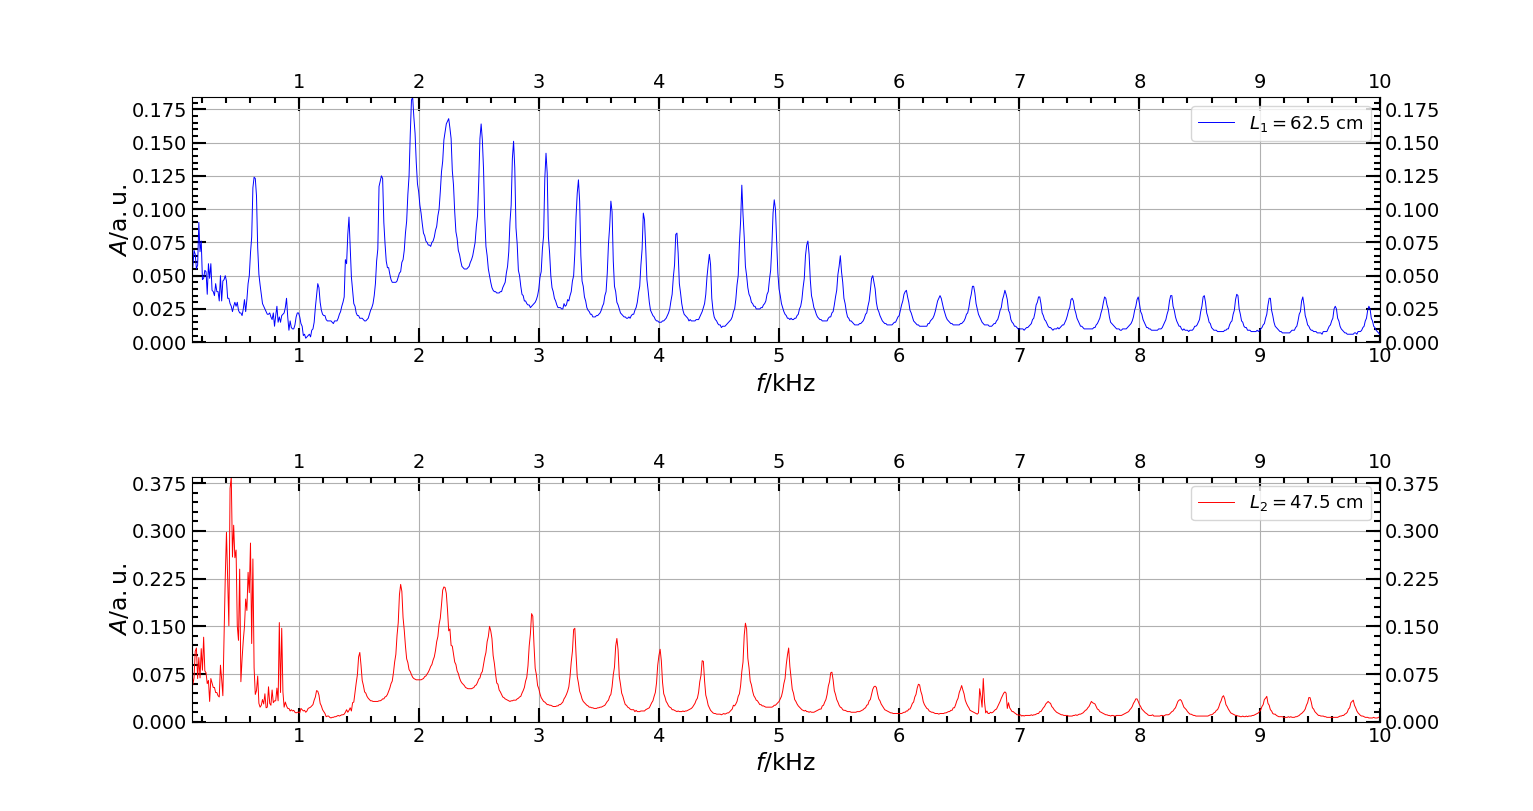
\includegraphics[width=0.9\textwidth]{421_Resonanzen.png} 
\caption{Frequenzspektrum für $L_1$ und $L_2$}
\end{figure} 
\[\]
\newpage
Es fällt auf, dass für die größere Länge die Abstände zwischen den Peaks kleiner sind. Dies hängt mit Gleichung (\ref{1}) zusammen. Umgestellt nach den Frequenzabständen $\Delta f$ der Peaks lautet diese nämlich:
\begin{align}
\Delta f = \frac{c}{2\,L} 
\end{align}
Unter der Annahme, dass die gleiche Schallgeschwindigkeit vorlag ist also $\Delta f$ umso größer, desto kleiner die Länge $L$. Außerdem sind diese immer äquidistant, was auch in obigem Plot zu erkennen ist.


Durch Durchnummerierung der ersten 20 Peaks mit $n=1,...,20$ konnten folgende Plots erstellt werden: 
\begin{figure}[h!]
\centering
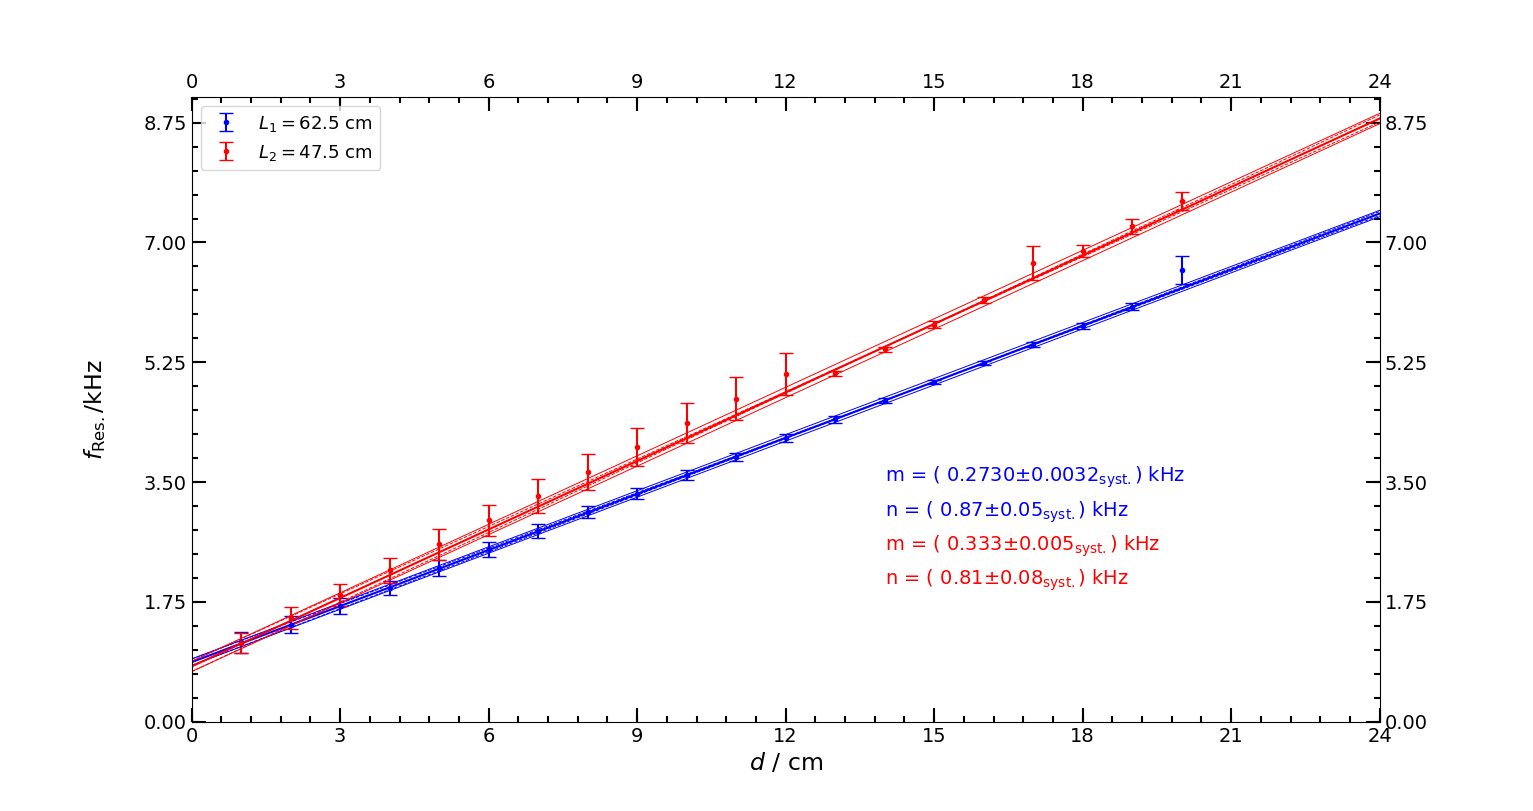
\includegraphics[width=0.85\textwidth]{421_systematische_Unsicherheiten.png} %hat nicht funktioniert
\caption{Ausgleichsgerade mit systematischen Unsicherheiten}
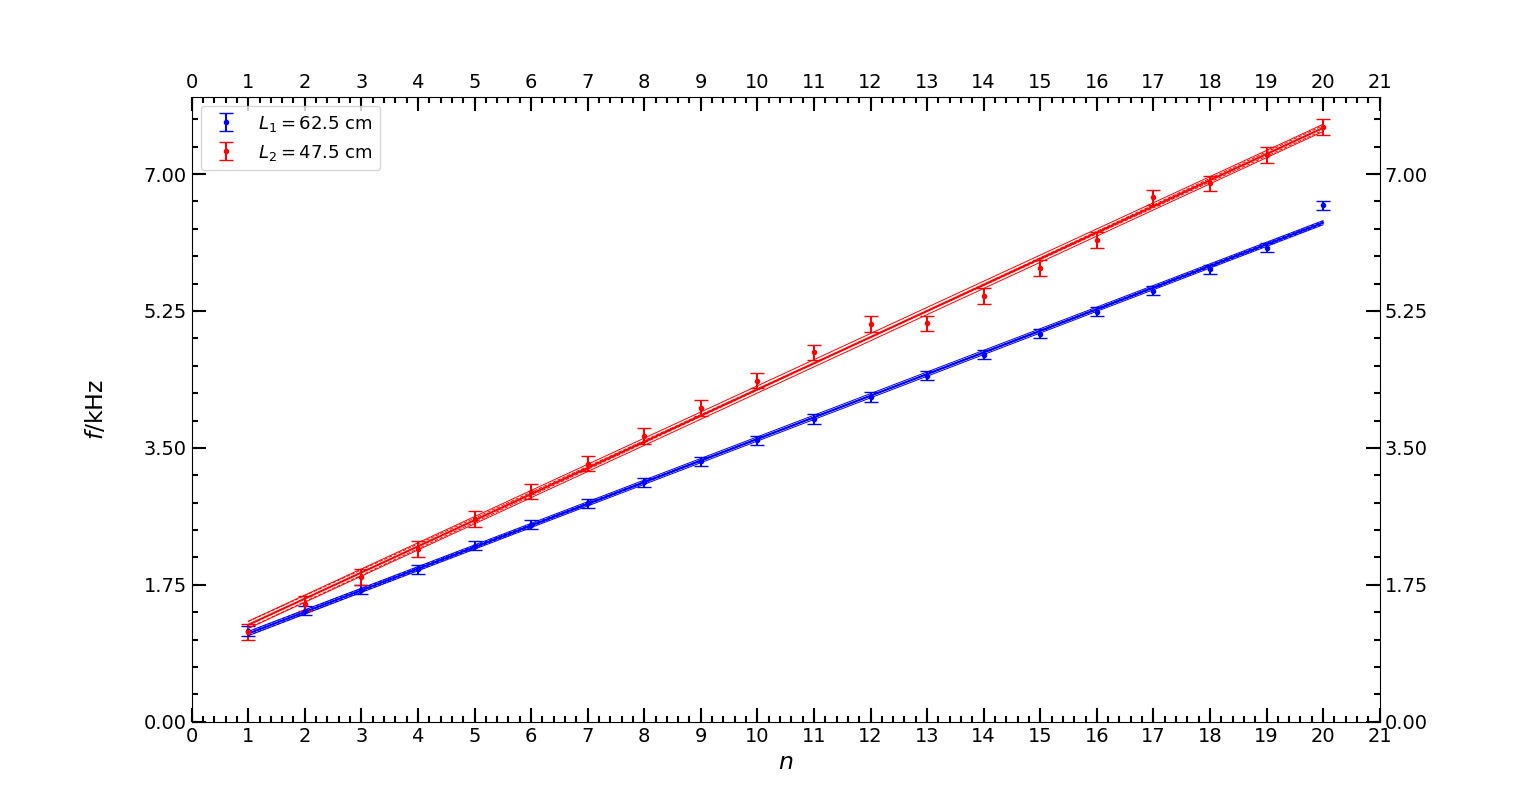
\includegraphics[width=0.85\textwidth]{421_statistische_Unsicherheiten.png} %hat nicht funktioniert
\caption{Ausgleichsgerade mit statistischen Unsicherheiten}
\end{figure} 
\newpage
Er stellt die Resonanzfrequenz in Abhängigkeit von der Nummer $n$ mit systematischer bzw. statistischer Unsicherheit dar. Daraus kann die Schallgeschwindigkeit aufgrund des Zusammenhangs (\ref{schall}) aus dem Anstieg bestimmt werden:
\begin{align}
\label{schall} f = n \cdot\frac{c_{\mathrm{Schall}}}{2L}
\end{align}
Man erhält also die experimentellen Werte für die Schallgeschwindigkeit aus dem Anstieg, indem man diesen mit $2L$ multipliziert. In diesem Fall ergaben sich die Schallgeschwindigkeiten zu:
\begin{align}
c_{\mathrm{Schall}}^{\mathrm{experimentell}} =
  \begin{cases}
    343,4 \pm 2,8_{\mathrm{stat.}} \pm 4,0_{\mathrm{sys.}}  & \text{für} \ L_{1}  \\
	317,1 \pm 3,7_{\mathrm{stat.}} \pm 5,0_{\mathrm{sys.}} & \text{für} \ L_{2}
  \end{cases}
\end{align}
Schließlich kann man die experimentell ermittelten Werte mit dem aus der Theorie errechneten Wert vergleichen. Der Wert für $L_1$ stimmt sehr gut mit dem Wert aus der Theorie überein. Der Wert für $L_2$ liegt allerdings weit von dem theoretischen Wert entfernt, selbst wenn man von den maximalen Unsicherheiten ausgeht. Dies könnte daran liegen, dass wie bereits diskutiert, für die kürzere Länge die Peaks breiter sind. Dies erschwert es die genaue Lage des Maximums zu bestimmen und bewirkt also eine zusätzliche Abweichung von der tatsächlichen Peak-Frequenz.
\newline
\newline Analog zum Teilchen im unendlich hohen Potential Topf kommt es also zur Ausbildung stehender Wellen im Resonator. Allerdings sind die Peaks im Resonator bezüglich der Frequenz äquidistant und die Energien $E(n)$ sind proportional zu $n^2$, also nicht äquidistant.

\subsubsection{Theoretisches Modell und Reproduzierbarkeit}
Um die Reproduzierbarkeit der Messung zu untersuchen wurden mit Hilfe eines Fit-Programms für 8 Peaks in einem Frequenzbereich von $1,6$ kHz bis $4,5$ kHz ein Fit vorgenommen. Dies ist im folgenden Plot dargestellt:
\begin{figure}[h!]
\centering
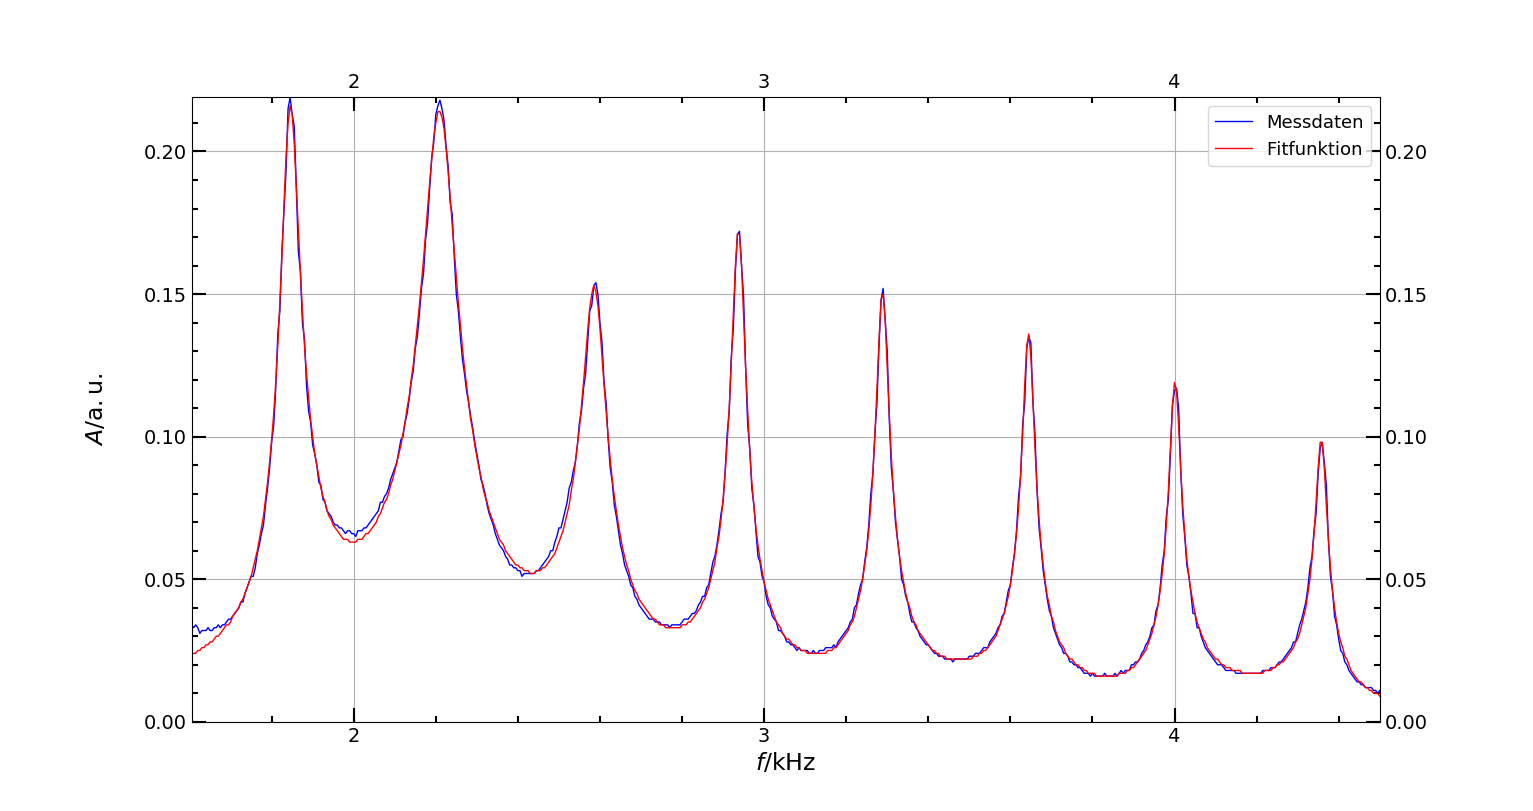
\includegraphics[width=0.7\textwidth]{Messung_L2_und_Fitfunktion.png}
\caption{Fit des theoretisches Modells zum experimentellen Spektrum}
\end{figure}
\newpage
Es ist also zu erkennen, dass dass das aufgenommene Frequenzspektrum sehr gut durch die im Fit-Programm verwendeten Gauß-Funktionen dargestellt werden können.
Somit ist die Reproduzierbarkeit und eine Übereinstimmung mit dem theoretischen Modell gegeben.

\subsection{Kugelresonator}
\subsubsection{Bestimmung der Resonanzfrequenzen und Winkelabhängigkeit der Wellenfunktion}
Nach Anpassung der Attentuator-Einstellung zur Signalabschwächung wurde ein Übersichtsspektrum zwischen $100$ Hz und $8$ kHz für einen Winkel $\alpha$ von $180^{\circ}$ (diese entspricht $\theta = 180^{\circ}$) aufgenommen. Dieses ist hier abgebildet: \\\\
\begin{figure}[h!]
\centering
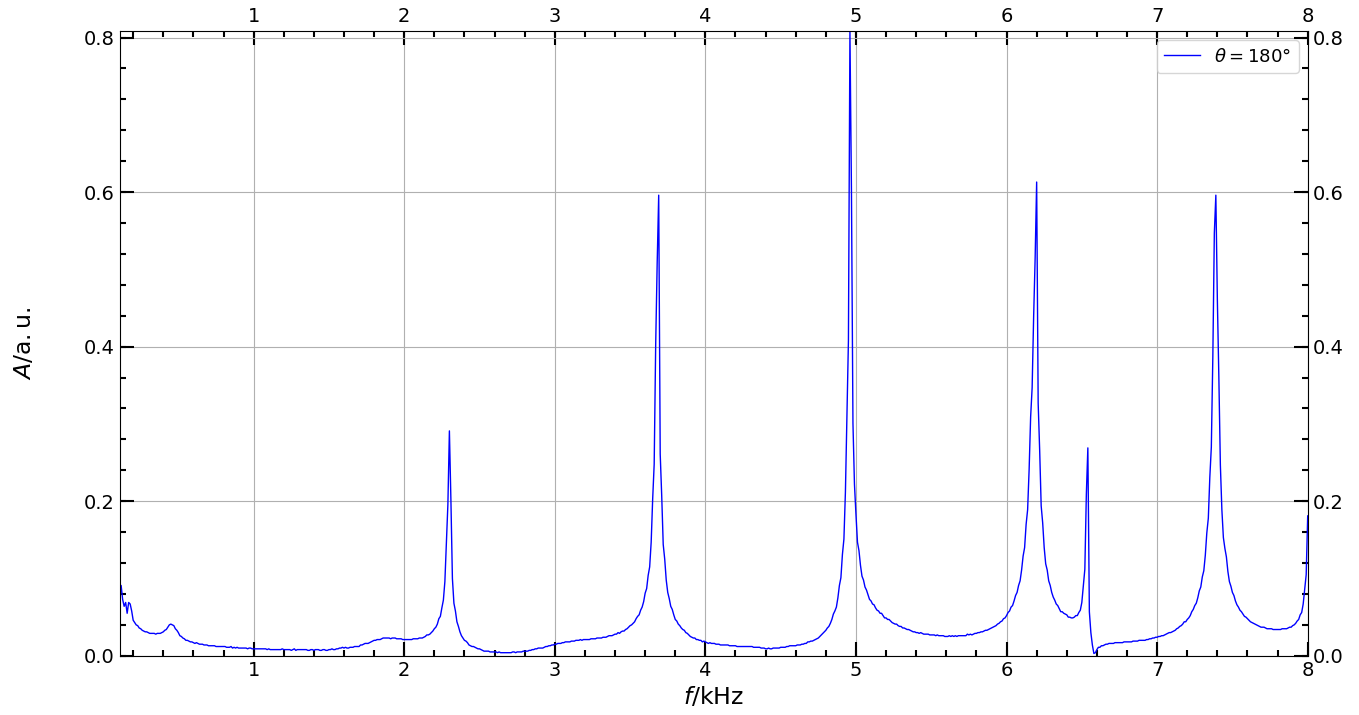
\includegraphics[width=\textwidth]{4311}
\caption{Übersichtsspektrum für $\alpha = \theta = 180^{\circ}$}
\end{figure}
Wieder ergaben sich Resonanzfrequenzen als Peaks. Diese lagen bei:

Diese Messung wurde für weitere Winkel $\alpha$ von  $0^{\circ}$, $60^{\circ}$, $85^{\circ}$ und $120^{\circ}$ wiederholt. Nach der gegebenen Vorschrift in $\theta$ umgerechnet lauten diese: $90^{\circ}$; $104,48^{\circ}$; $117,16^{\circ}$ und $138,59^{\circ}$. Die 4 Spektren sind in folgendem Plot zur besseren Vergleichbarkeit zusammen dargestellt: \\\\
\begin{figure}[h!]
\centering
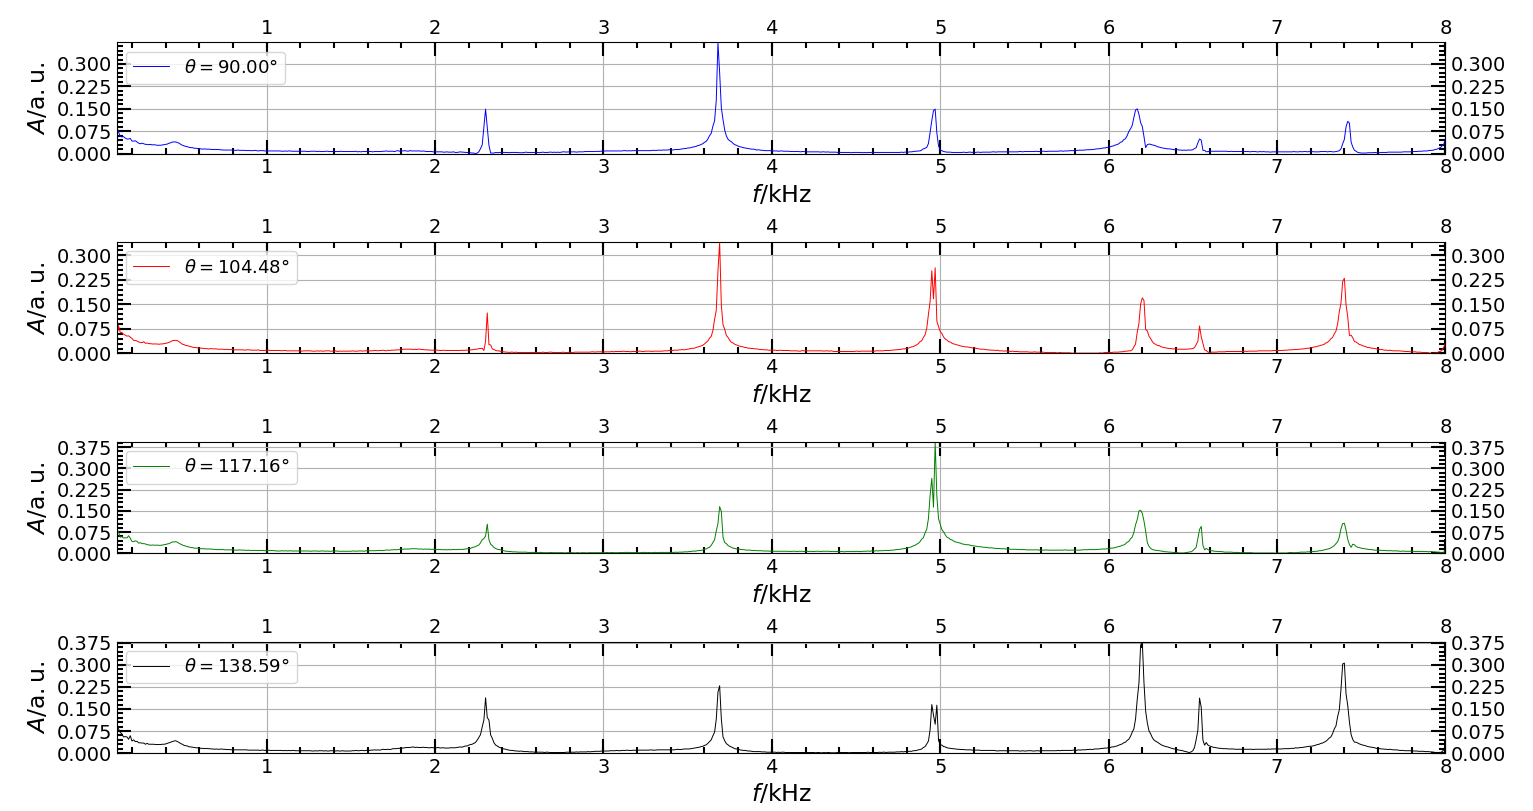
\includegraphics[width=\textwidth]{4312}
\caption{Frequenzspektren für verschiedene Winkel $\theta$}
\end{figure}






\subsubsection{Polardiagramme}








    % Bibliographie/Literaturverzeichnis
    \begin{thebibliography}{9}
    \bibitem{wiki:Intensität}
    Wikipedia,
    \emph{Intensität (Physik)},
    \url{https://de.wikipedia.org/wiki/Intensit%C3%A4t_(Physik)},
    25.\,Okt.~2019.
    \end{thebibliography}
% Ende Dokument

\end{document}
